\documentclass[15pt]{article}
\usepackage[utf8]{inputenc}
\usepackage{natbib}
\usepackage{graphicx}
\usepackage{float}
\usepackage{array}
\usepackage{tabularx}
\usepackage{geometry}
\usepackage{titlesec}
\usepackage{sectsty}
\usepackage{enumitem}
\usepackage{lipsum}
\usepackage{longtable}
\usepackage{booktabs,xltabular}
\usepackage{setspace}
\usepackage{tocloft,lipsum,pgffor,sectsty}
\usepackage{tocbasic}
\usepackage[font=Large,labelfont=bf]{caption}
\usepackage{enumitem}
\usepackage[toc,page]{appendix}
\usepackage{hyperref}
\hypersetup{
    colorlinks=true,
    linkcolor=black,
    filecolor=black,      
    urlcolor=blue,
    anchorcolor = black,
    citecolor=black
}

 \geometry{
 a4paper,
 total={170mm,257mm},
 left=20mm,
 top=20mm,
 }

\titleformat*{\section}{\LARGE\bfseries}
\titleformat*{\subsection}{\tiny\bfseries}
\titleformat*{\subsubsection}{\large\bfseries}
\titleformat*{\paragraph}{\large\bfseries}
\titleformat*{\subparagraph}{\large\bfseries}

\begin{document}

\begin{titlepage}

\addtolength{\hoffset}{-0.1cm}
	\centering
	
\includegraphics[width=0.60\textwidth]{logo.png}\par\vspace{1.5cm}
	{\huge\bfseries SOEN 6481 \par}
	{\huge\bfseries Software Systems Requirements Specification \par}
	{\scshape\LARGE Fall 2019 \par}
	\vspace{1cm}
	\vspace{1.5cm}
	{\huge\bfseries Ticket Vending Machine \par}
	{\huge\bfseries Requirements Specification \par}
	\vspace{1cm}
	{\scshape\LARGE Team F \par}

	\vspace{0.5cm}
	\begin{tabular}{ c l }
	\vspace{0.2cm}
	{\Large\bfseries 40083289 \par} & {\Large Dhaval Chandreshkumar Modi \par}\\
	\vspace{0.2cm}
	{\Large\bfseries 40084358 \par} & {\Large Dolly Modha  \par}\\
	\vspace{0.2cm}
	{\Large\bfseries 40085480 \par} & {\Large Liangzhao Lin  \par}\\
	\vspace{0.2cm}
	{\Large\bfseries 40082567 \par} & {\Large Naren Morabagal Somasekhar \par}\\
	\vspace{0.2cm}
	{\Large\bfseries 40076735 \par} & {\Large Pruthvi Raju Nallaparaju \par}\\
	\end{tabular}
	\vspace{0.5cm}

    \vspace{0.5cm}

	\vfill

	\vspace{0.2cm}
	{\large Supervised By} \par
    \vspace{0.2cm}
	{\Large Prof. Pankaj Kamthan}

	\vfill
	{\Large Google Drive : \url{http://bit.ly/2ON5C1C}\par}
	\vspace{0.2cm}
    {\Large Github Repo: \url{http://bit.ly/2IQRBMt}}

	\vfill

% Bottom of the page
	{\large \today\par}
	\par
    
\end{titlepage}


\renewcommand{\cftpartfont}{\Large\bfseries}
\renewcommand\cftsecfont{\Large\bfseries}
\renewcommand\cftsecpagefont{\Large\bfseries}
\renewcommand{\cftsubsecfont}{\Large\bfseries}
\renewcommand{\cftsubsecpagefont}{\Large\bfseries}
\renewcommand\cftsecafterpnum{\par\addvspace{6pt}}
\renewcommand\cftloftitlefont{\Large\bfseries}
\renewcommand\cftfigfont{\Large\bfseries}
\renewcommand\cftfigpagefont{\Large\bfseries}




\doublespacing
\tableofcontents
\singlespacing
\setlength{\cftparskip}{1\baselineskip}
\listoffigures

\subsectionfont{\Large}



\newpage
\section{\Large{Introduction}}
\subsection{\Large{Description}}
\Large{The primary functionality of TVM (Ticket Vending Machine) is to accept request from the user and to print out a ticket\cite{fernandes2016requirements}. Taking inspiration from the current version of the TVM that has been implemented by STM, in our TVM we decided to give options for purchasing a ticket in five different possibilities. One trip ticket, Two trip Ticket, One day pass, Weekly Pass and Monthly Pass. At the end of our project, our main goal is to develop functional software which offers functionalities similar to the Montreal metro TVM\cite{kulak2012use}. Our secondary goal is to propose upgradation(if any) upon the functional or non-functional requirements implementation of Montreal metro TVM.}
\subsection{\Large{Why we chose this Project?}}
At the inception, the Montreal metro-line only covered 26 stations with 3 lines\cite{chan2013station}. But today, it connects 68 stations with five different lines. The number of stations has been more than doubled. They added these stations without affecting the established stations. In accordance with the physical changes in the metro lines, there needs to add more requirements in the ticketing software. In other words ticketing software has also evolved with the Montreal Metro transportation system. In this way, TVM ticketing software, had mimicked the software development evolution life-cycle. As the software evolves with time, there needs to be taken care of the current requirements and adding more without affecting the functionalities of the current version. One of the best approach which can define this process is the ’Iterative Software Development Model’. Planning, Requirements gathering, Design,  Implementation, Testing and Evaluation are the important stages in this development model. These stages not only correlates to the software system but also it applies similarly to the growth pattern of Metro in physical world.\par
Moreover, looking at the complexity and the scale of the project, it would be interesting to analyze all the functional, nonfunctional requirements and design TVM Software\citep{alexander2009discovering}.
\subsection{\Large{The Future}}
From the past, what we can predict is that with the economic growth of Montreal, there will be more stations to be added in upcoming years. Keeping these modifications in mind, we will try to design the TVM software which will be easy to maintain as well as easy to add new requirements\cite{laplante2017requirements}.


\section{\Large{Context of Use Model}}

\begin{center}
\begin{longtable}{| p{.40\textwidth} | p{.60\textwidth} |} 
 \hline
  {\bfseries Types of factors}\citep{dey2001understanding} & {\bfseries Attributes} \\ [0.5ex] 
 \hline
 User & 
 \begin{itemize}
  \item Age
  \item Past Usage
  \item Language
  \item Skills
  \item Mental/Physical Capabilities
  \item Other Requirements
  \end{itemize}  \\ 
 \hline
 
User Task
 &  \begin{itemize}
  \item Criticality of Task
  \item Task-Specific Goals
  \item Dependency
  \item Usage Time
  \item Risks
  \end{itemize}   \\
 \hline
 
User Activities
 &  \begin{itemize}
  \item Constraints
  \end{itemize}   \\
 \hline
 
 User Task
 &  \begin{itemize}
  \item Criticality of Task
  \item Task-Specific Goals
  \item Dependency
  \item Usage Time
  \item Risks
  \end{itemize}   \\
 \hline

Location and Time
 &  \begin{itemize}
  \item Time-Zone
  \item Location
  \end{itemize}   \\
 \hline
 
Issues due to Nature
 &  \begin{itemize}
  \item Light
  \item Temperature
  \end{itemize}   \\
 \hline
 
Technical Requirements
 &  \begin{itemize}
  \item Hardware
    \begin{itemize}
        \item  Processor Speed
        \item Screen
        \item Keyboard
    \end{itemize}
  \item Software
    \begin{itemize}
        \item Operating System
        \item Server
    \end{itemize}
  \end{itemize}   \\
 \hline
 
 
 
Social Environment
 &  \begin{itemize}
  \item Legal Constraints
  \end{itemize}   \\
 [1ex] 
 \hline
\end{longtable}
\end{center}
\vspace{1cm}
\subsection{\Large{ Description of contextual Use factors}}

\begin{enumerate}[leftmargin=2em, itemsep=0pt, parsep=0pt, , font=\Large\bfseries]
    \item {\Large\bfseries User}
        \begin{itemize}
            \item {\Large\bfseries Age} : Age is one of the constraints for the user since children under 10 years old cannot travel on their own.
            \item {\Large\bfseries Past usage } : No need of using the TVM previously since the machine displays all the commands to be followed by the user.
            \item {\Large\bfseries Language} : User should be able to read either English/French.
            \item {\Large\bfseries Skills} : User can use the machine even though; he does not have command on computer language.
            \item {\Large\bfseries Mental/Physical capabilities} : A person should be mentally stable and should be able to use his/her hand. But a blind person can use the TVM with the help of braille script on the keys.
            \item {\Large\bfseries Other Requirements} : A person should have the patience to stand in the queue.
        \end{itemize}
        \vspace{1cm}
    \item {\Large\bfseries User Task}
        \begin{itemize}
            \item {\Large\bfseries Criticality of Task} : The process is followed in steps one followed by another so that it becomes easier for the user. In addition, there should be clarity about the task.
            \item {\Large\bfseries Task-Specific Goals} : Firstly, accept the money from the user in the form of cash or card payment then ticket is generated after the card is recharged.
            \item {\Large\bfseries Dependency} : Connections at the backend with the network in order to process the bank transactions, power connection and the paper to print the details of the payment.
            \item {\Large\bfseries Usage Time} : User can buy a ticket from 5:30am to 11pm according to the stm rules. Exclusion of standing in the line a user requires two minutes for the complete successful process.
            \item {\Large\bfseries Risks} : There are few risks involved like entering the wrong details of the card by user, during payment by the bank.
        \end{itemize}
    \item {\Large\bfseries User Activities}
        \begin{itemize}
                \item {\Large\bfseries Constraints} : User must be more than 4 feet in order to use the TVM and he/she needs to tilt the screen in order to use it sitting in the wheelchair.
        \end{itemize}
    \item {\Large\bfseries Location and Time}
        \begin{itemize}
            \item {\Large\bfseries Time-zone} : TVM follows eastern time zone since it is installed in Montreal.
            \item {\Large\bfseries Location} : TVM should be placed in a bigger space so that there won’t be any problem even though people stand in queue. In addition, it should be placed at the entrance.
        \end{itemize}
    \item {\Large\bfseries Issues due to Nature}
        \begin{itemize}
            \item {\Large\bfseries Light} : TVM screen adjust the screen even when it is dark.
            \item {\Large\bfseries Temperature} : Machine should be able to work in any climate regardless of sunny or windy or rainy.
        \end{itemize}
    \item {\Large\bfseries Technical Requirements}
        \begin{itemize}
            \item {\Large\bfseries Hardware}
                \begin{itemize}
                    \item {\Large\bfseries Processor speed} : Should be fast enough so that TVM handles all the processes efficiently.
                    \item {\Large\bfseries Screen} : Touch screen with proper LED display.
                    \item {\Large\bfseries Keyboard} : Interactive keyboard that has the numbers and other buttons. It has an added advantage of braille script for the blind.
                \end{itemize}
            \item {\Large\bfseries Software}
                \begin{itemize}
                    \item {\Large\bfseries Operating System} : software should be user friendly and reliable.
                    \item {\Large\bfseries Server} : Requires server in order to backup the data.
                \end{itemize}
        \end{itemize}
    \item {\Large\bfseries Social Environment}
    \begin{itemize}
            \item {\Large\bfseries Legal constraints} : Installation and utilization of TVM must be approved by the government.
        \end{itemize}
\end{enumerate}



\newpage
\section{\Large{ Problem Domain model}}

\begin{figure}[H]
\centering
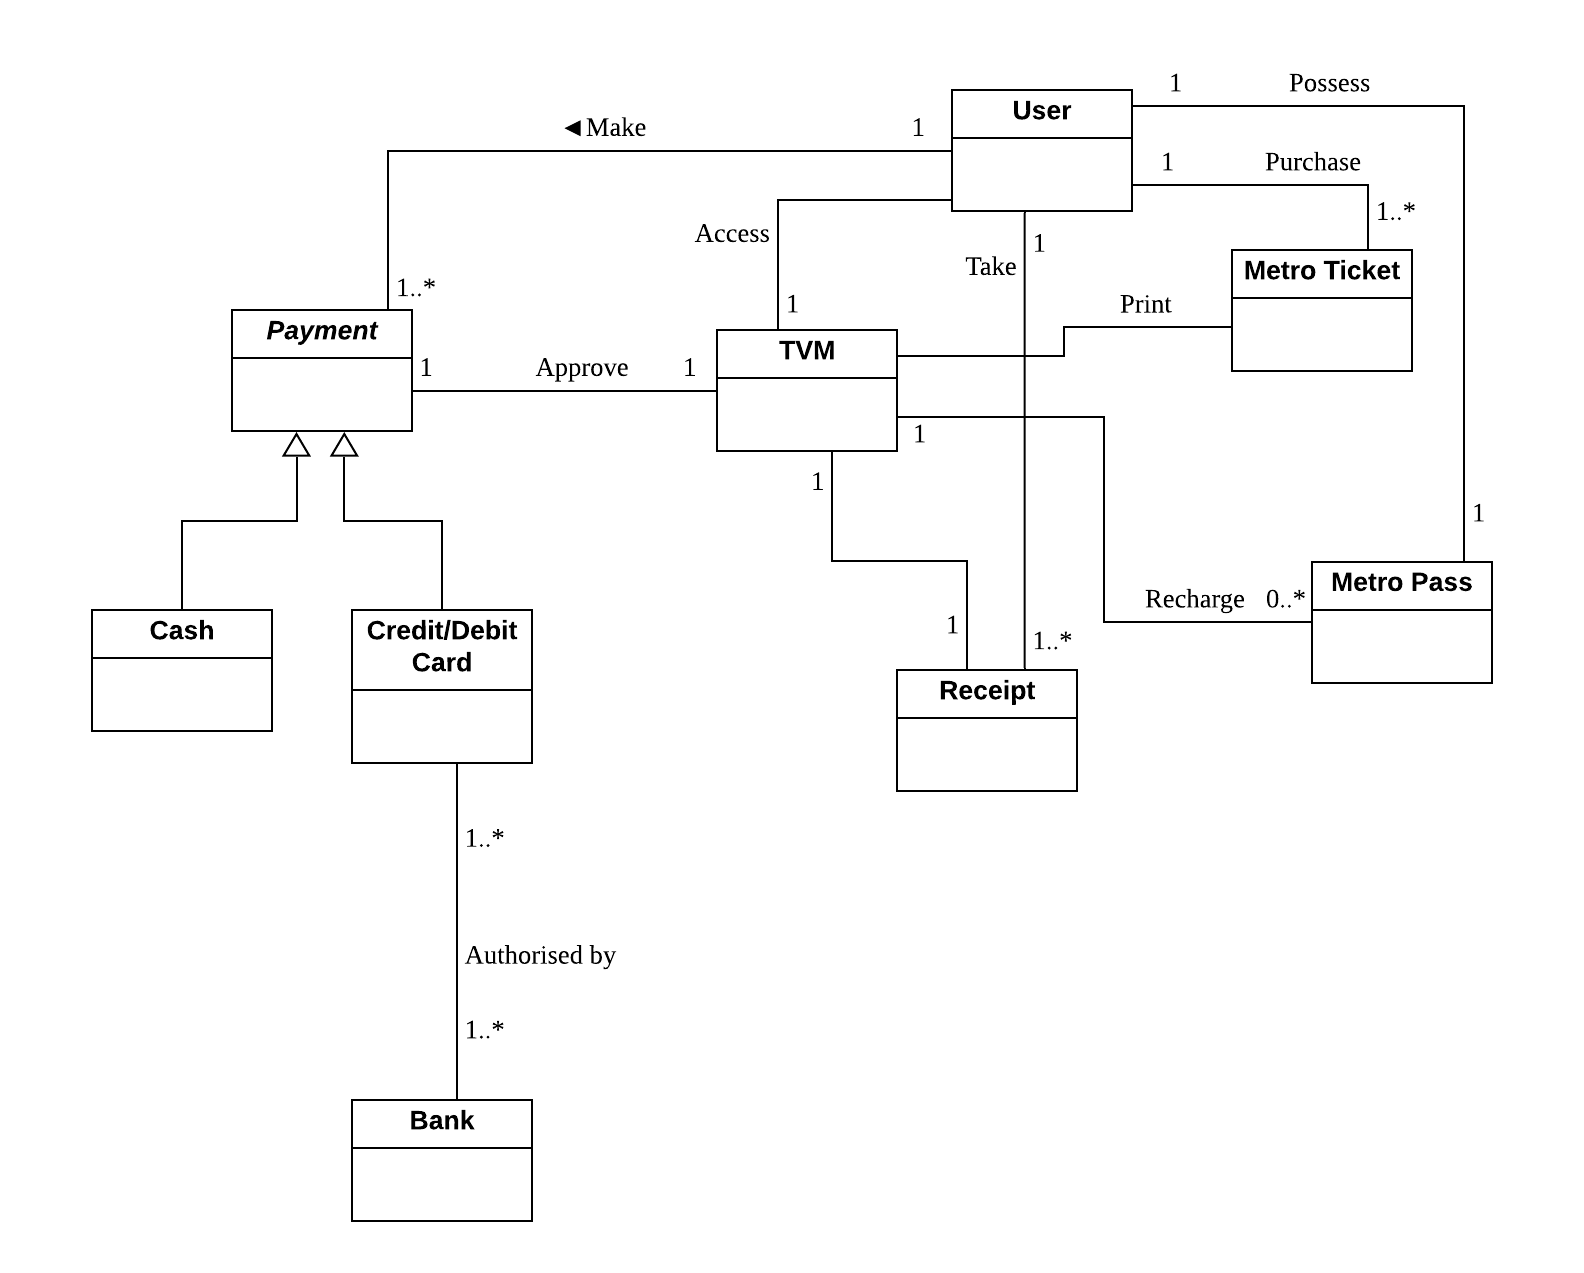
\includegraphics[scale=0.4]{domain.png}
\caption{\Large\bfseries{Problem Domain Model\cite{prieto1991domain}}}
\label{Problem Domain Model:do}
\end{figure}

\subsection{\Large{Description of TVM concept}}
        \begin{itemize}
            \item {\Large\bfseries User} : The person who uses the ticket vending machine to buy the desired metro ticket or recharge the metro pass.
            \item {\Large\bfseries Bank } : An external system authorise the debit/credit used by the user.
            \item {\Large\bfseries Payment} : The user pays through this concept, have two options that pay in cash and pay in credit or debit card.
            \item {\Large\bfseries TVM} : TVM is a ticket vending machine, which is a system for users to purchase metro tickets.
            \item {\Large\bfseries Metro Ticket} : Tickets for users to take the metro, there are four types:one-trip, two-trip, day pass and weekly pass.
            \item {\Large\bfseries Metro Pass} : This is the metro recharge card, which is a chip integrated plastic made. Users can directly use the metro card to enter the metro station ticket, and it is recharged through TVM.
             \item {\Large\bfseries Receipt} : Receipt of the purchase printed by TVM after payment by the user.
        \end{itemize}
 

\subsection{\Large{Description of relationship between the concepts}}
        \begin{itemize}
            \item {\Large\bfseries User - TVM} : A user access only one ticket vending machine and purchase follow the system's process.
            \item {\Large\bfseries User - Receipt } : A user can take one to many receipts for one day pass, weekly pass.
            \item {\Large\bfseries User - Metro Ticket} : A user can take one to many tickets.
            \item {\Large\bfseries User - Metro Pass} : A user can take only one metro pass. As he/she can recharge it anytime when required.
            \item {\Large\bfseries User - Payment} :  A user can do one to many payments.
            \item {\Large\bfseries TVM - Metro Ticket} : One to many tickets can be printed by TVM.
             \item {\Large\bfseries TVM - Metro Pass} : There can only be one pass per user.
             \item {\Large\bfseries TVM - Receipt} : One to many tickets can be generated.
            \item {\Large\bfseries TVM - Payment } : One to many payments can be done.
            \item {\Large\bfseries Payment - Cash} : A Cash payment is a subclass of payment and it adds behaviour to payment class to pay by Cash.
            \item {\Large\bfseries Payment - Credit/Debit Card} : A Credit/Debit Card payment is a subclass of payment and it adds behaviour to payment class to pay by Credit/Debit Card.
            \item {\Large\bfseries Credit/Debit Card - Bank} : Credit/Debit card is inherited from bank.
        \end{itemize}       
        
        
\section{\Large{Use Case Diagram}}

\begin{figure}[H]
\centering
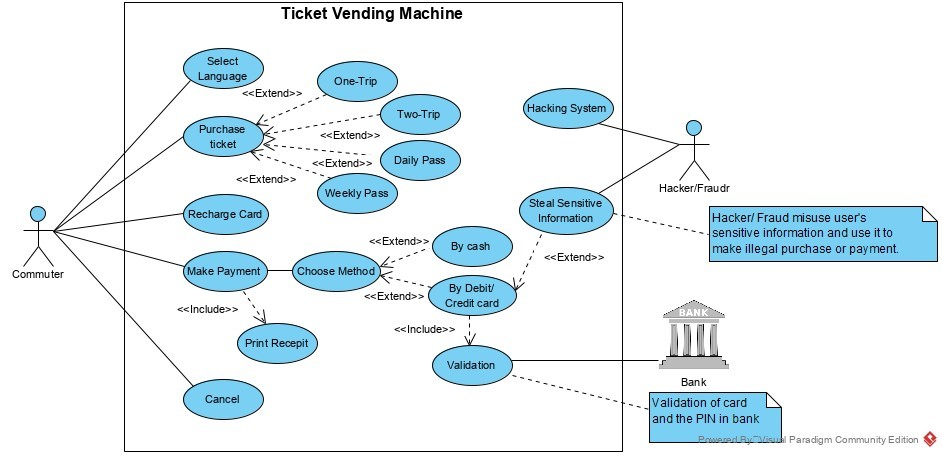
\includegraphics[scale=0.7]{Use_Case.jpg}
\caption{\Large\bfseries{Use Case Diagram\cite{umlpk}}}
\label{Use Case Diagram:do}
\end{figure}

Use case model involves mainly two actors namely Commuter and Ticket Vending Machine. Com    muter use cases involve selection of language, purchasing of ticket, recharging of card, make payment for ticket/card. Whereas, TVM takes care of the displaying types of tickets, internal connection to the bank. Apart from these actors, there are two more actors namely Bank which takes care of the payment transactions and a negative use case actor, Hacker who hacks the system and steals the user data.

\newpage

\subsection{\Large{Fully Dressed Use case Scenarios}}
 \begin{enumerate}[leftmargin=2em, itemsep=0pt, parsep=0pt, , font=\Large\bfseries]
 \item {\Large\bfseries{Language Selection}} : Commuter upon reaching the TVM selects his/her required language from the available languages and TVM displays the language chosen by Commuter.
\newline
\newline
\begin{tabularx}{1\textwidth} { 
  | >{\raggedright\arraybackslash}X 
  | >{\raggedright\arraybackslash}X 
  | }
 \hline
 Use Case & UC01 Language selection \\
 Priority & High \\
 Primary Actor  & User \\
 Secondary Actor  & TVM \\

 Pre-Condition  & 
 \begin{enumerate}
  \item Display the instructions to select a language to continue by the languages supported by the TVM.
  \end{enumerate}
  \\
  
   Post-condition  & \begin{enumerate}
  \item The interface will display the ticket selection information in selected language.
  \end{enumerate}
  \\
  
  Steps/ Flow  & \begin{enumerate}
  \item  TVM displays the instructions to select a language.
  \item TVM user selects a language to continue.
  \end{enumerate}
  \\
  
   Additional or Exception flow/s  & \begin{enumerate}
  \item  Cancel process.
  \end{enumerate}
  \\
    
   Success Scenario  & \begin{enumerate}
  \item  The user selects his/her preferred language on the menu.
  \item  TVM displays ticket selection information in the selected language.
  \end{enumerate}
  \\

\hline
\end{tabularx}


\newpage
\item {\Large\bfseries{Ticket Selection Mode}} : After the selection of language TVM displays a message whether to purchase the ticket or recharge the card.
\newline
\newline
\begin{tabularx}{1\textwidth} { 
  | >{\raggedright\arraybackslash}X 
  | >{\raggedright\arraybackslash}X 
  | }
 \hline
 Use Case & UC02 Select Purchase ticket or Recharge card \\
 Priority & High \\
 Primary Actor  & User \\
 Secondary Actor  & TVM \\

 Pre-Condition  & 
 \begin{enumerate}
  \item The user has selected the language.
  \end{enumerate}
  \\
  
   Post-condition  & \begin{enumerate}
  \item User has opted either to purchase ticket or recharge card.
  \end{enumerate}
  \\
  
  Steps/ Flow  & \begin{enumerate}
  \item TVM displays the instructions to select a language.
  \item The user selects the preferred language.
  \item TVM displays options to purchase ticket and recharge card in the selected language.
  \item  The user selects either purchase ticket or recharge card.
  \end{enumerate}
  \\
  
   Additional or Exception flow/s  & \begin{enumerate}
  \item  Cancel process.
  \end{enumerate}
  \\
    
   Success Scenario  & \begin{enumerate}
  \item  The user opts to purchase his/her ticket, or to recharge card.
  \item  TVM displays an interface for purchase tickets or recharge cards.
  \end{enumerate}
  \\

\hline
\end{tabularx}



\newpage
\item {\Large\bfseries{Purchasing a ticket}} : TVM displays available tickets from where he/she can select the ticket from the available options.
\newline
\newline
\begin{figure}[H]
\centering
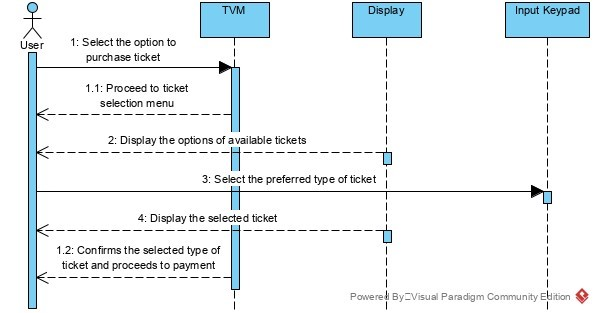
\includegraphics[width=\textwidth,height=\textheight,keepaspectratio]{Purchase_Ticket_seq.jpg}
\caption{\Large\bfseries{Purchase Ticket Sequence Diagram}}
\label{Purchase Ticket Sequence Diagram:do}
\end{figure}

This sequence diagram shows the sequence of actions between the objects in order to purchase a ticket by Commuter.

\begin{tabularx}{1\textwidth} { 
  | >{\raggedright\arraybackslash}X 
  | >{\raggedright\arraybackslash}X 
  | }
 \hline
 Use Case & UC03 Purchase Ticket \\
 Priority & High \\
 Primary Actor  & User \\
 Secondary Actor  & TVM \\

 Pre-Condition  & 
 \begin{enumerate}
  \item The user has opted to purchase the ticket.
  \end{enumerate}
  \\
  
   Post-condition  & \begin{enumerate}
  \item The user has selected his/her preferred type of ticket and proceeds to pay for the ticket.
  \end{enumerate}
  \\
  
  Steps/ Flow  & \begin{enumerate}
  \item  TVM displays options to purchase ticket or recharge card.
  \item The user selects the option to purchase the ticket.
  \item TVM displays options to buy a ticket for either one-trip, 2-trip, daily or weekly pass.
  \item  The user selects his/her preferred ticket.
  \item The user proceeds to make payment.
  \end{enumerate}
  \\
  
   Additional or Exception flow/s  & \begin{enumerate}
  \item  Change selected ticket type.
  \item  Change the ticket selection mode to recharge card.
  \item  Cancel process.
  \end{enumerate}
  \\
    
   Success Scenario  & \begin{enumerate}
  \item  Preferred ticket selected successfully.
  \item  Proceeds to make payment.
  \end{enumerate}
  \\

\hline
\end{tabularx}


\newpage
\item {\Large\bfseries{Recharging the card}} : In this Use Case Commuter inserts the card after the selecting purchase ticket option, TVM starts the payment process for the commuter.
\newline
\newline
\begin{tabularx}{1\textwidth} { 
  | >{\raggedright\arraybackslash}X 
  | >{\raggedright\arraybackslash}X 
  | }
 \hline
 Use Case &  UC04 Recharge card \\
 Priority &  Medium/ Moderate \\
 Primary Actor  & User \\
 Secondary Actor  & TVM \\

 Pre-Condition  & 
 \begin{enumerate}
  \item The user inserts the card.
  \item Selects the option to recharge card.
  \end{enumerate}
  \\
  
   Post-condition  & \begin{enumerate}
  \item The user confirms to recharge card and proceeds to make payment.
  \end{enumerate}
  \\
  
  Steps/ Flow  & \begin{enumerate}
  \item  TVM display the option to purchase ticket or recharge card.
  \item The user selects the option to recharge card.
  \item TVM displays the option to recharge card.
  \item  The user confirms to recharge card.
  \item The user proceeds to make payment.
  \end{enumerate}
  \\
  
   Additional or Exception flow/s  & \begin{enumerate}
  \item  Change the ticket selection mode to purchase the ticket.
  \item  Cancel process.
  \end{enumerate}
  \\
    
   Success Scenario  & \begin{enumerate}
  \item The user confirmed to recharge the card.
  \item Proceeds to make payment.
  \end{enumerate}
  \\

\hline
\end{tabularx}



\newpage
\item {\Large\bfseries{Selecting the Payment option}} : From the options available like payment by cash or payment by card commuter chooses his/her mode of payment.
\newline
\newline
\begin{tabularx}{1\textwidth} { 
  | >{\raggedright\arraybackslash}X 
  | >{\raggedright\arraybackslash}X 
  | }
 \hline
 Use Case & UC05 Select Payment Mode \\
 Priority & High \\
 Primary Actor  & User \\
 Secondary Actor  & TVM \\

 Pre-Condition  & 
 \begin{enumerate}
  \item The user has selected their ticket type or to reload the card.
  \item Confirms for payment.
  \end{enumerate}
  \\
  
   Post-condition  & \begin{enumerate}
  \item The user has selected the mode of payment and proceeds to pay in the chosen method.
  \end{enumerate}
  \\
  
  Steps/ Flow  & \begin{enumerate}
  \item TVM displays the options for different modes of payment by cash or debit/credit card.
  \item The user select his/her preferred option of payment.
  \item The user proceeds to make payment by cash or by debit/credit card.
  \end{enumerate}
  \\
  
   Additional or Exception flow/s  & \begin{enumerate}
  \item  Change payment mode.
  \item  Cancel process.
  \end{enumerate}
  \\
    
   Success Scenario  & \begin{enumerate}
  \item Confirms payment mode and proceeds to make payment.
  \end{enumerate}
  \\

\hline
\end{tabularx}



\newpage
\item {\Large\bfseries{Payment by Cash}} : Commuter chooses the option to pay by cash.
\newline
\newline
\begin{tabularx}{1\textwidth} { 
  | >{\raggedright\arraybackslash}X 
  | >{\raggedright\arraybackslash}X 
  | }
 \hline
 Use Case & UC06 Pay by Cash \\
 Priority & High \\
 Primary Actor  & User \\
 Secondary Actor  & TVM \\

 Pre-Condition  & 
 \begin{enumerate}
  \item The user has opted to make payment by cash.
  \end{enumerate}
  \\
  
   Post-condition  & \begin{enumerate}
  \item Payment made successfully.
  \item Dispense ticket and payment receipt.
  \end{enumerate}
  \\
  
  Steps/ Flow  & \begin{enumerate}
  \item TVM displays a message to make payment by cash.
  \item User makes payment by inserting cash into the TVM.
  \item TVM confirms payment has been done.
  \item TVM dispense ticket and payment receipt.
  \end{enumerate}
  \\
  
   Additional or Exception flow/s  & \begin{enumerate}
  \item  TVM returns the difference amount back to the user. 
  \end{enumerate}
  \\
    
   Success Scenario  & \begin{enumerate}
  \item Payment made successfully.
  \item Ticket and payment receipt is dispensed.
  \item In case of return change, it is returned back to the user.
  \end{enumerate}
  \\

\hline
\end{tabularx}


\newpage
\item {\Large\bfseries{Payment by Card}} : Commuter chooses the option to pay by either credit or debit card.
\newline
\begin{xltabular}{1\textwidth} { 
  | >{\raggedright\arraybackslash}X 
  | >{\raggedright\arraybackslash}X 
  | }
 \hline
 Use Case &  UC07 Pay by Debit/Credit card \\
 Priority & High \\
 Primary Actor  & User \\
 Secondary Actor  & TVM and Bank \\

 Pre-Condition  & 
 \begin{enumerate}
  \item The user has opted to make payment by Debit/Credit card.
  \end{enumerate}
  \\
  
   Post-condition  & \begin{enumerate}
  \item Payment made successfully.
  \item Dispense ticket and payment receipt.
  \end{enumerate}
  \\
  
  Steps/ Flow  & \begin{enumerate}
  \item TVM displays a message to make payment by card.
  \item User makes payment by inserting  Debit/Credit card into the TVM.
  \item TVM communicates with bank to validate the card.
  \item TVM asks the user to enter the PIN to complete the payment.
  \item The user enters the PIN.
  \item Once again, TVM communicates with bank to validate the PIN.
  \item TVM confirms payment has been done.
  \item TVM dispense ticket and payment receipt.
  \item The user takes back his/her card.
  \end{enumerate}
  \\
  
   Additional or Exception flow/s  & \begin{enumerate}
  \item  TVM cancels payment and transactions in case of failed validation. 
  \end{enumerate}
  \\
    
   Success Scenario  & \begin{enumerate}
  \item Payment made successfully.
  \item Ticket and payment receipt is dispensed.
  \item In case of return change, it is returned back to the user.
  \end{enumerate}
  \\

\hline
\end{xltabular}


\vspace{2cm}
\begin{figure}[H]
\centering
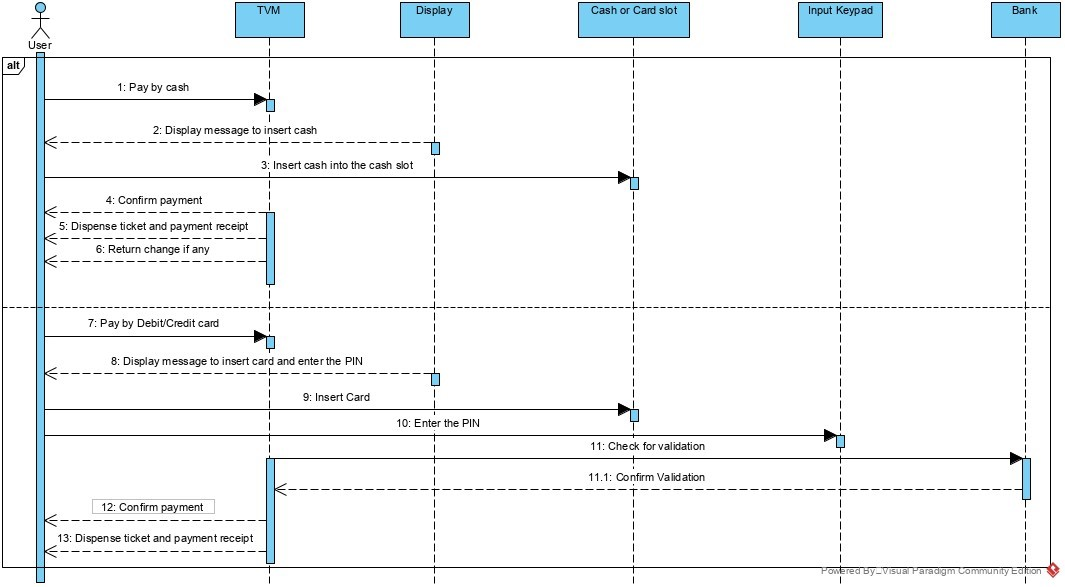
\includegraphics[width=\textwidth,height=\textheight,keepaspectratio]{Payment_Seq.jpg}
\caption{\Large\bfseries{Payment Sequence Diagram}}
\label{Payment Sequence Diagram:do}
\end{figure}
This sequence diagram shows how the sequence of actions carried out in order for the Commuter to pay the amount either by cash or a card.






\newpage
\item {\Large\bfseries{Cancel Transaction Process}} : Transaction may get cancelled if the user does not have enough balance or entered an incorrect pin.
\newline
\newline
\begin{tabularx}{1\textwidth} { 
  | >{\raggedright\arraybackslash}X 
  | >{\raggedright\arraybackslash}X 
  | }
 \hline
 Use Case &   UC08 Cancel transaction process \\
 Priority & High \\
 Primary Actor  & User \\
 Secondary Actor  & TVM \\

 Pre-Condition  & 
 \begin{enumerate}
  \item The user is not on the homepage.
  \item The user is unaware of the transaction process
  \end{enumerate}
  \\
  
   Post-condition  & \begin{enumerate}
  \item The transaction process is canceled and return to the homepage.
  \end{enumerate}
  \\
  
  Steps/ Flow  & \begin{enumerate}
  \item User is currently not in Homepage.
  \item The user clicks cancel button.
  \item TVM cancels the transaction and takes the user back to Homepage.
  \end{enumerate}
  \\
  
   Additional or Exception flow/s  & \begin{enumerate}
  \item  The user decides not to use TVM, cancels process and walks away.
  \end{enumerate}
  \\
    
   Success Scenario  & \begin{enumerate}
  \item  User is unaware about transaction or want to change selection.
  \item The transaction is cancelled.
  \item TVM takes the user back to the homepage.
  \end{enumerate}
  \\

\hline
\end{tabularx}


\newpage
\item {\Large\bfseries{Misuse of User Sensitive Information}} : This is a special use case where a new actor named Hacker is involved where he/she retrieves the TVM data in order to misuse the user data.
\newline
\newline
\begin{tabularx}{1\textwidth} { 
  | >{\raggedright\arraybackslash}X 
  | >{\raggedright\arraybackslash}X 
  | }
 \hline
 Use Case & UC09 Theft/ Misuse of user’s sensitive information \\
 Priority & High \\
 Primary Actor  & Hacker \\
 Secondary Actor  & TVM \\

 Pre-Condition  & 
 \begin{enumerate}
  \item  The user has inserted the card and entered the PIN.
  \end{enumerate}
  \\
  
   Post-condition  & \begin{enumerate}
  \item The TVM system is hacked and user’s privacy is violated.
  \end{enumerate}
  \\
  
  Steps/ Flow  & \begin{enumerate}
  \item Enters and runs in the system unethically.
  \item Performs operations to retrieve user’s sensitive information.
  \item Violate user’s privacy.
  \end{enumerate}
  \\
  
   Additional or Exception flow/s  & \begin{enumerate}
  \item  Perform illegal operations and steal data.
  \end{enumerate}
  \\

\hline
\end{tabularx}

\newpage
\item {\Large\bfseries{Payment Fraud}} :  It is similar to Misuse use case. Upon retrieving the user banking information, hacker move the money paid by Commuter to a third party. 
\newline
\newline
\begin{tabularx}{1\textwidth} { 
  | >{\raggedright\arraybackslash}X 
  | >{\raggedright\arraybackslash}X 
  | }
 \hline
 Use Case &   UC10 Payment Fraud \\
 Priority & High \\
 Primary Actor  & Hacker \\
 Secondary Actor  & TVM \\

 Pre-Condition  & 
 \begin{enumerate}
  \item  The user has inserted the card and entered the PIN.
  \end{enumerate}
  \\
  
   Post-condition  & \begin{enumerate}
  \item The TVM system is hacked and money is stolen. 
  \end{enumerate}
  \\
  
  Steps/ Flow  & \begin{enumerate}
  \item Enters and runs in the system unethically.
  \item The system is hacked and the user’s banking information is stolen.
  \item A 3rd-party/ hacker receives the payment.
  \end{enumerate}
  \\
  
   Additional or Exception flow/s  & \begin{enumerate}
  \item  Perform illegal operations and steal money.
  \end{enumerate}
  \\

\hline
\end{tabularx}
\end{enumerate}

\subsection{\Large{Activity Diagram}}

\begin{figure}[H]
\centering
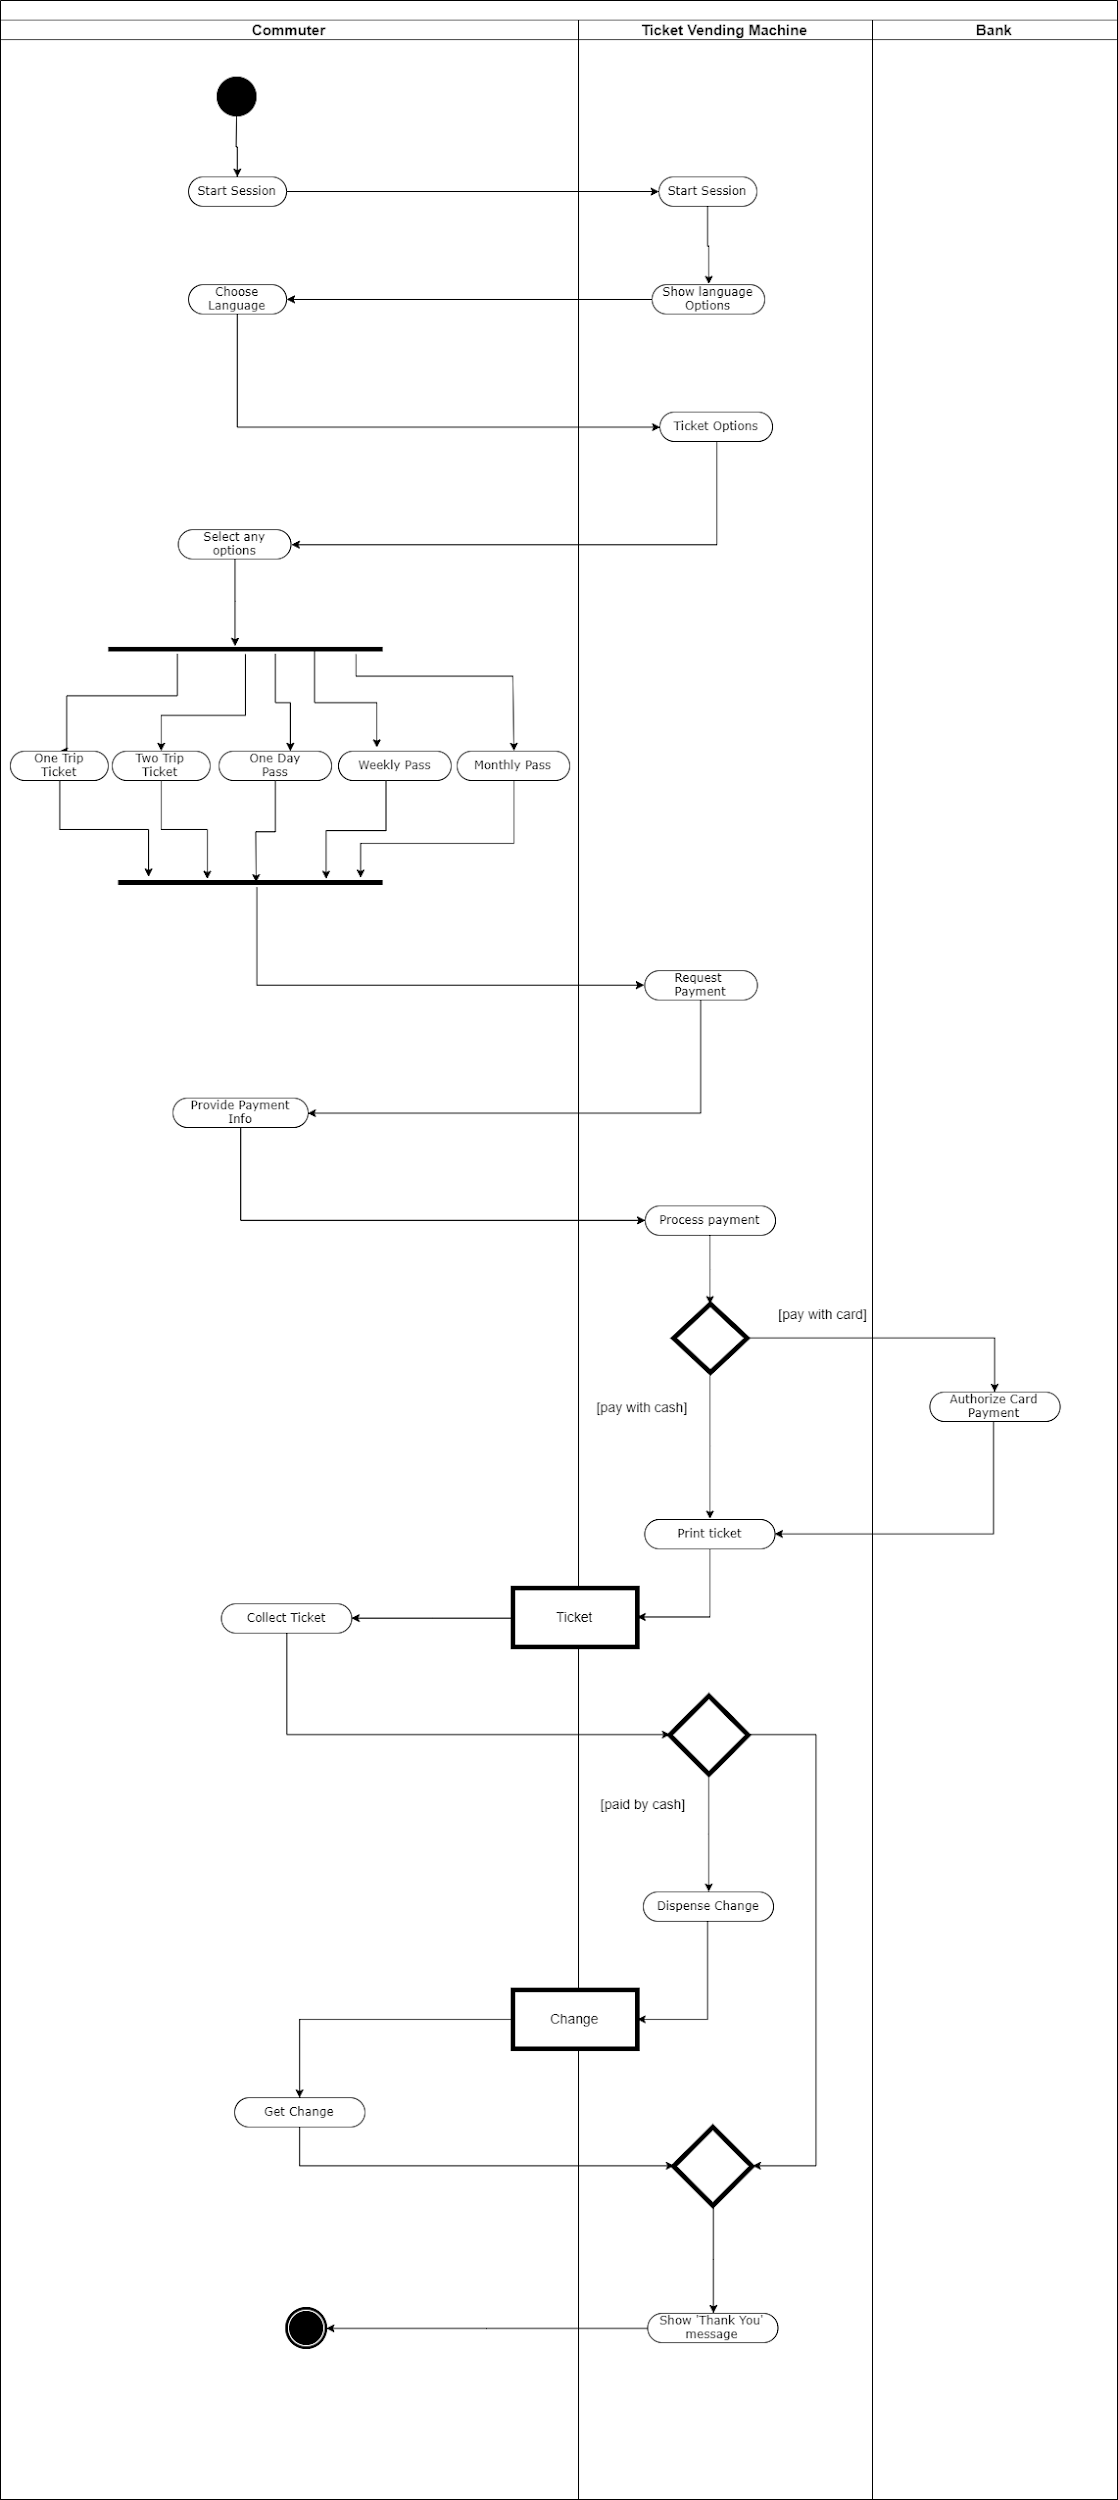
\includegraphics[width=250pt,height=\textheight,keepaspectratio]{Activity_Diagram.png}
\caption{\Large\bfseries{Activity Diagram}}
\label{Activity Diagram:do}
\end{figure}

In the above given activity diagram, Commuter is the one who will start the activity. After the session has been started, he/she will request for the trip information from the TVM on the screen, it will show different options in which a user can purchase a ticket. For our scenario, he/she will be shown five different options. According to the needs of the commuter, he/she will choose the option. Based on the selection, TVM calculates the amount to be paid. It will then after shows different options using which a commuter can pay for the ticket. If he/she pays by cash, he will get back the change. And if he/she chooses to pay by card, bank intervention is needed to confirm if the payment is successful or not. After the successful payment, TVM will print out the ticket. At the end of this activity, TVM shows ‘Thank You’ message. 


\begin{appendices}
\addtocontents{toc}{\protect\setcounter{tocdepth}{0}}
\section*{Interview Transcript}

\begin{enumerate}[leftmargin=3em, itemsep=0pt, parsep=0pt, , font=\Large\bfseries]
    \item {\Large\bfseries Interview with Runsen Tian}
    \begin{enumerate}[leftmargin=2em, itemsep=0pt, parsep=0pt, , font=\Large\bfseries]
        \item {\Large Which language do you prefer to operate the TVM?}
        \vspace{0.1cm}
            \begin{itemize}
                \item {\Large I prefer English.}
            \end{itemize}
            \vspace{0.2cm}
        \item {\Large How often do you commute in the metro?}
        \vspace{0.1cm}
            \begin{itemize}
                \item {\Large I travel for my school and for my work too. So, usually on a daily basis I commute.}
            \end{itemize}
            \vspace{0.2cm}
        \item {\Large Do you prefer using a rechargeable card or purchasing tickets?}
        \vspace{0.1cm}
            \begin{itemize}
                \item {\Large  According to me, Rechargeable card will be preferable.}
            \end{itemize}
            \vspace{0.2cm}
        \item {\Large Which type of ticket do you prefer, one-trip, 2-trip, daily pass, weekly pass?}
        \vspace{0.1cm}
            \begin{itemize}
                \item {\Large I prefer daily pass.}
            \end{itemize}
            \vspace{0.2cm}
        \item {\Large Why this particular type of ticket?}
        \vspace{0.1cm}
            \begin{itemize}
                \item {\Large As I commute daily, so I prefer the daily pass.}
            \end{itemize}
            \vspace{0.2cm}
        \item {\Large In your opinion, how easy or difficult is the TVM to operate?}
        \vspace{0.1cm}
            \begin{itemize}
                \item {\Large I feel it is quite easy as it does not have any other features.}
            \end{itemize}
            \vspace{0.2cm}
        \item {\Large Which mode of payment do you prefer, by cash or by debit/credit card?}
            \begin{itemize}
                \item {\Large I prefer the credit/debit card.}
            \end{itemize}
            \vspace{0.2cm}
        \item {\Large Have you faced any issues when making the payment?}
        \vspace{0.1cm}
            \begin{itemize}
                \item {\Large No, I have not faced any issues till now.}
            \end{itemize}
            \vspace{0.2cm}
        \item {\Large Have you ever had a feeling of not using the TVM, so you canceled your transaction and walked away?}
        \vspace{0.1cm}
            \begin{itemize}
                \item {\Large Yes, it happened one time when there was a long queue.}
            \end{itemize}
            \vspace{0.2cm}
    \end{enumerate}
    
    
    \vspace{0.2cm}
    \item {\Large\bfseries Interview with Shreya Monpara}\\
    \begin{enumerate}[leftmargin=2em, itemsep=0pt, parsep=0pt, , font=\Large\bfseries]
        \item {\Large Which language do you prefer to operate the TVM?}
        \vspace{0.1cm}
            \begin{itemize}
                \item {\Large I prefer French.}
            \end{itemize}
            \vspace{0.2cm}
        \item {\Large How often do you commute in the metro?}
        \vspace{0.1cm}
            \begin{itemize}
                \item {\Large I travel for my work. So, usually on a daily basis I commute.}
            \end{itemize}
            \vspace{0.2cm}
        \item {\Large Do you prefer using a rechargeable card or purchasing tickets?}
        \vspace{0.1cm}
            \begin{itemize}
                \item {\Large  Recharging  a card is a good idea.}
            \end{itemize}
            \vspace{0.2cm}
        \item {\Large Which type of ticket do you prefer, one-trip, 2-trip, daily pass, weekly pass?}
        \vspace{0.1cm}
            \begin{itemize}
                \item {\Large I prefer daily pass.}
            \end{itemize}
            \vspace{0.2cm}
        \item {\Large Why this particular type of ticket?}
        \vspace{0.1cm}
            \begin{itemize}
                \item {\Large I feel it is quite easy as it does not have any more steps.}
            \end{itemize}
            \vspace{0.2cm}
        \item {\Large In your opinion, how easy or difficult is the TVM to operate?}
        \vspace{0.1cm}
            \begin{itemize}
                \item {\Large I feel it is quite easy as it does not have any other features.}
            \end{itemize}
            \vspace{0.2cm}
        \item {\Large Which mode of payment do you prefer, by cash or by debit/credit card?}
            \begin{itemize}
                \item {\Large I prefer the credit/debit card.}
            \end{itemize}
            \vspace{0.2cm}
        \item {\Large Have you faced any issues when making the payment?}
        \vspace{0.1cm}
            \begin{itemize}
                \item {\Large No, I have not faced any issues till now.}
            \end{itemize}
            \vspace{0.2cm}
        \item {\Large Have you ever had a feeling of not using the TVM, so you canceled your transaction and walked away?}
        \vspace{0.1cm}
            \begin{itemize}
                \item {\Large No, I always recharge my card one day prior to the new month so I never came across rushing through TVM.}
            \end{itemize}
            \vspace{0.2cm}
    \end{enumerate}
    
    
    \vspace{0.2cm}
    \item {\Large\bfseries Interview with TA}\\
    \begin{enumerate}[leftmargin=2em, itemsep=0pt, parsep=0pt, , font=\Large\bfseries]
        \item {\Large Which language do you prefer to operate the TVM?}
        \vspace{0.1cm}
            \begin{itemize}
                \item {\Large I prefer English.}
            \end{itemize}
            \vspace{0.2cm}
        \item {\Large How often do you commute in the metro?}
        \vspace{0.1cm}
            \begin{itemize}
                \item {\Large I do not commute via metro.}
            \end{itemize}
            \vspace{0.2cm}
        \item {\Large Do you prefer using a rechargeable card or purchasing tickets?}
        \vspace{0.1cm}
            \begin{itemize}
                \item {\Large  Purchasing a ticket as I do not commute by metro.}
            \end{itemize}
            \vspace{0.2cm}
        \item {\Large Which type of ticket do you prefer, one-trip, 2-trip, daily pass, weekly pass?}
        \vspace{0.1cm}
            \begin{itemize}
                \item {\Large I prefer one day pass.}
            \end{itemize}
            \vspace{0.2cm}
        \item {\Large Why this particular type of ticket?}
        \vspace{0.1cm}
            \begin{itemize}
                \item {\Large I do not travel in metro.}
            \end{itemize}
            \vspace{0.2cm}
        \item {\Large In your opinion, how easy or difficult is the TVM to operate?}
        \vspace{0.1cm}
            \begin{itemize}
                \item {\Large I feel it as easy going work.}
            \end{itemize}
            \vspace{0.2cm}
        \item {\Large Which mode of payment do you prefer, by cash or by debit/credit card?}
            \begin{itemize}
                \item {\Large I prefer cash.}
            \end{itemize}
            \vspace{0.2cm}
        \item {\Large Have you faced any issues when making the payment?}
        \vspace{0.1cm}
            \begin{itemize}
                \item {\Large No, I have not faced any issues till now.}
            \end{itemize}
            \vspace{0.2cm}
        \item {\Large Have you ever had a feeling of not using the TVM, so you canceled your transaction and walked away?}
        \vspace{0.1cm}
            \begin{itemize}
                \item {\Large No, As I am not using that much of commuting through metro.}
            \end{itemize}
            \vspace{0.2cm}
    \end{enumerate}
    
    
    \vspace{0.2cm}  
    \item {\Large\bfseries Interview with Sukesh Mudrakola}\\
    \begin{enumerate}[leftmargin=2em, itemsep=0pt, parsep=0pt, , font=\Large\bfseries]
        \item {\Large Which language do you prefer to operate the TVM?}
        \vspace{0.1cm}
            \begin{itemize}
                \item {\Large I prefer English.}
            \end{itemize}
            \vspace{0.2cm}
        \item {\Large How often do you commute in the metro?}
        \vspace{0.1cm}
            \begin{itemize}
                \item {\Large I commute a lot in metro. As I have my residence, school and metro everything near metro station.}
            \end{itemize}
            \vspace{0.2cm}
        \item {\Large Do you prefer using a rechargeable card or purchasing tickets?}
        \vspace{0.1cm}
            \begin{itemize}
                \item {\Large  Recharging a card is the best option for me.}
            \end{itemize}
            \vspace{0.2cm}
        \item {\Large Which type of ticket do you prefer, one-trip, 2-trip, daily pass, weekly pass?}
        \vspace{0.1cm}
            \begin{itemize}
                \item {\Large I prefer daily pass.}
            \end{itemize}
            \vspace{0.2cm}
        \item {\Large Why this particular type of ticket?}
        \vspace{0.1cm}
            \begin{itemize}
                \item {\Large As said, I travel a lot.}
            \end{itemize}
            \vspace{0.2cm}
        \item {\Large In your opinion, how easy or difficult is the TVM to operate?}
        \vspace{0.1cm}
            \begin{itemize}
                \item {\Large I feel it as a very easy task.}
            \end{itemize}
            \vspace{0.2cm}
        \item {\Large Which mode of payment do you prefer, by cash or by debit/credit card?}
            \begin{itemize}
                \item {\Large I prefer debit card.}
            \end{itemize}
            \vspace{0.2cm}
        \item {\Large Have you faced any issues when making the payment?}
        \vspace{0.1cm}
            \begin{itemize}
                \item {\Large No, I have not faced any issues till now.}
            \end{itemize}
            \vspace{0.2cm}
        \item {\Large Have you ever had a feeling of not using the TVM, so you canceled your transaction and walked away?}
        \vspace{0.1cm}
            \begin{itemize}
                \item {\Large Yes, As people are always in a hurry for the metro so many times I come again in the late night or early morning to recharge my card.}
            \end{itemize}
            \vspace{0.2cm}
    \end{enumerate}
    
    \vspace{0.2cm}
    \item {\Large\bfseries Interview with Devarsh Modi}\\
    \begin{enumerate}[leftmargin=2em, itemsep=0pt, parsep=0pt, , font=\Large\bfseries]
        \item {\Large Which language do you prefer to operate the TVM?}
        \vspace{0.1cm}
            \begin{itemize}
                \item {\Large I prefer English.}
            \end{itemize}
            \vspace{0.2cm}
        \item {\Large How often do you commute in the metro?}
        \vspace{0.1cm}
            \begin{itemize}
                \item {\Large I commute daily  either for my work or my school.}
            \end{itemize}
            \vspace{0.2cm}
        \item {\Large Do you prefer using a rechargeable card or purchasing tickets?}
        \vspace{0.1cm}
            \begin{itemize}
                \item {\Large  I recharge my card every time.}
            \end{itemize}
            \vspace{0.2cm}
        \item {\Large Which type of ticket do you prefer, one-trip, 2-trip, daily pass, weekly pass?}
        \vspace{0.1cm}
            \begin{itemize}
                \item {\Large I prefer daily pass.}
            \end{itemize}
            \vspace{0.2cm}
        \item {\Large Why this particular type of ticket?}
        \vspace{0.1cm}
            \begin{itemize}
                \item {\Large  It is cheaper so I prefer daily pass.}
            \end{itemize}
            \vspace{0.2cm}
        \item {\Large In your opinion, how easy or difficult is the TVM to operate?}
        \vspace{0.1cm}
            \begin{itemize}
                \item {\Large There is no any issues in operating TVM.}
            \end{itemize}
            \vspace{0.2cm}
        \item {\Large Which mode of payment do you prefer, by cash or by debit/credit card?}
            \begin{itemize}
                \item {\Large I prefer credit card.}
            \end{itemize}
            \vspace{0.2cm}
        \item {\Large Have you faced any issues when making the payment?}
        \vspace{0.1cm}
            \begin{itemize}
                \item {\Large No, I have not faced any issues.}
            \end{itemize}
            \vspace{0.2cm}
        \item {\Large Have you ever had a feeling of not using the TVM, so you canceled your transaction and walked away?}
        \vspace{0.1cm}
            \begin{itemize}
                \item {\Large Yes, I think it’s easy but it's tedious sometimes so I go to Ticket Vendors.}
            \end{itemize}
            \vspace{0.2cm}
    \end{enumerate}
    
    
    \vspace{0.2cm}   
    \item {\Large\bfseries Interview with Jaldhi Prajapati}\\
    \begin{enumerate}[leftmargin=2em, itemsep=0pt, parsep=0pt, , font=\Large\bfseries]
        \item {\Large Which language do you prefer to operate the TVM?}
        \vspace{0.1cm}
            \begin{itemize}
                \item {\Large I prefer English.}
            \end{itemize}
            \vspace{0.2cm}
        \item {\Large How often do you commute in the metro?}
        \vspace{0.1cm}
            \begin{itemize}
                \item {\Large I commute daily for my school.}
            \end{itemize}
            \vspace{0.2cm}
        \item {\Large Do you prefer using a rechargeable card or purchasing tickets?}
        \vspace{0.1cm}
            \begin{itemize}
                \item {\Large  I recharge my card every time.}
            \end{itemize}
            \vspace{0.2cm}
        \item {\Large Which type of ticket do you prefer, one-trip, 2-trip, daily pass, weekly pass?}
        \vspace{0.1cm}
            \begin{itemize}
                \item {\Large I prefer daily pass.}
            \end{itemize}
            \vspace{0.2cm}
        \item {\Large Why this particular type of ticket?}
        \vspace{0.1cm}
            \begin{itemize}
                \item {\Large  It is cheaper so I prefer daily pass.}
            \end{itemize}
            \vspace{0.2cm}
        \item {\Large In your opinion, how easy or difficult is the TVM to operate?}
        \vspace{0.1cm}
            \begin{itemize}
                \item {\Large There is no any issues in operating TVM.}
            \end{itemize}
            \vspace{0.2cm}
        \item {\Large Which mode of payment do you prefer, by cash or by debit/credit card?}
            \begin{itemize}
                \item {\Large I prefer credit card.}
            \end{itemize}
            \vspace{0.2cm}
        \item {\Large Have you faced any issues when making the payment?}
        \vspace{0.1cm}
            \begin{itemize}
                \item {\Large I never faced any issues while operating TVM.}
            \end{itemize}
            \vspace{0.2cm}
        \item {\Large Have you ever had a feeling of not using the TVM, so you canceled your transaction and walked away?}
        \vspace{0.1cm}
            \begin{itemize}
                \item {\Large Yes, because sometimes I think that recharging a card is a bad idea else do Uber and commute.}
            \end{itemize}
            \vspace{0.2cm}
    \end{enumerate}
    
\end{enumerate}
\end{appendices}

\bibliographystyle{plain}
\bibliography{references}
\end{document}
